\documentclass[a4paper]{article}
\usepackage{graphicx}
\usepackage{amsmath,amssymb}
\usepackage{hyperref}
\usepackage{minted}
\usepackage{multirow}
\usepackage{float}
\usepackage{tikz}
\usetikzlibrary{mindmap}
\input{/home/donkarlo/Dropbox/repo/nd_ai_project/src/nd_ai/language/formal/computer/programming/tex/composition/control_sequence/kind/tag/tag.tex}

\title{Mindmap}
\date{}

\begin{document}
    \maketitle
    
    
    \section{Mindmap}
        \begin{figure}[H]
            \raggedright
            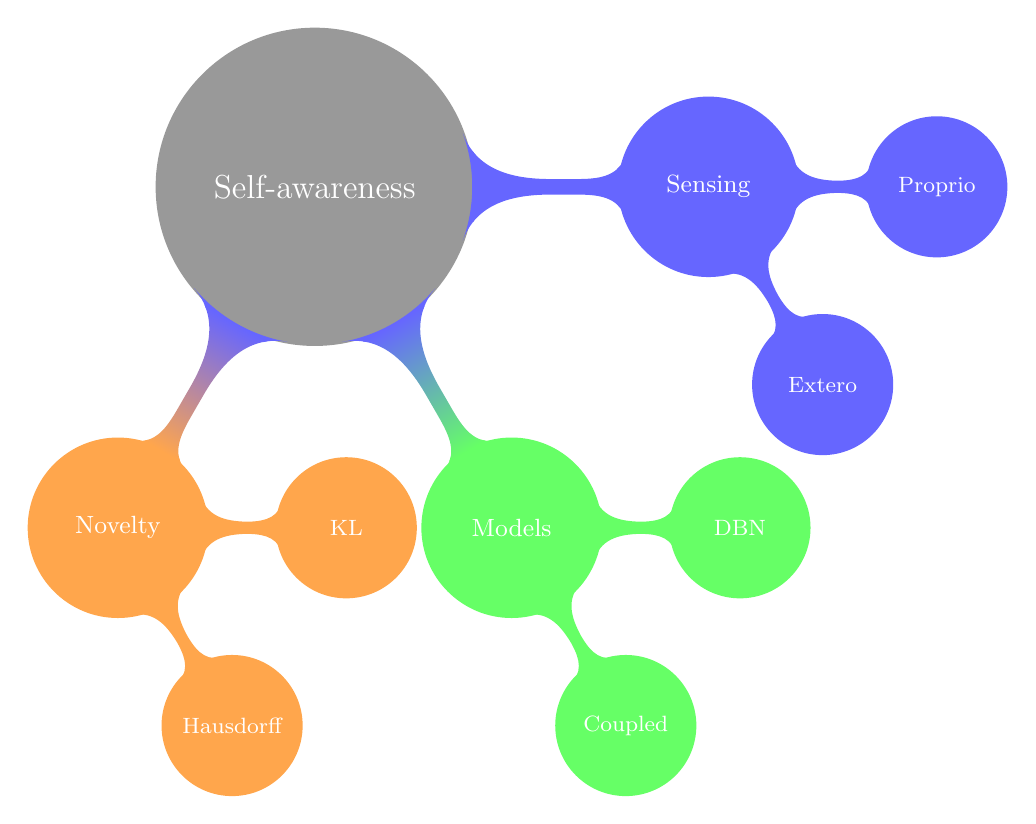
\begin{tikzpicture}
                \path[mindmap,concept color=black!40,text=white]
                node[concept] {Self-awareness}
                [clockwise from=0, level 1 concept/.append style={concept color=blue!60}]
                child[concept color=blue!60] { node[concept] {Sensing}
                child { node[concept] {Proprio} }
                child { node[concept] {Extero} } }
                child[concept color=green!60] { node[concept] {Models}
                child { node[concept] {DBN} }
                child { node[concept] {Coupled} } }
                child[concept color=orange!70] { node[concept] {Novelty}
                child { node[concept] {KL} }
                child { node[concept] {Hausdorff} } };
            \end{tikzpicture}
            \caption{Mindmap of self-awareness}
            \label{fig:mindmap}
        \end{figure}
    % \bibliographystyle{plain}
    % \bibliography{/home/donkarlo/Dropbox/repo/shared_research/bibliography/bibliography.bib}
\end{document}